\colorlet{species background color}{black!15}
\tikzset{
    x={1pt},
    y={-1pt},
    species background/.style={
        fill=species background color,
        draw=species background color,
        line width={1pt},
    },
    species label/.style={
        font=\bfseries,
        midway,
        anchor=west,
        align=left,
        xshift=10,
    },
    branch/.style={
        draw={#1},
        line width={0.5pt},
    },
    transfer branch/.style={
        branch={#1},
        -Stealth,
    },
    loss/.style={
        draw={#1}, cross out, thick,
        line width={0.5pt},
        inner sep=0pt,
        outer sep=0pt,
        minimum width={3},
        minimum height={3},
    },
    extant gene/.style 2 args={
        circle, fill={#1},
        outer sep=0pt, inner sep=0pt,
        minimum size={3},
        label={
            [font={\color{#1}},
                align=justify,
                inner xsep=4pt, inner ysep=0pt,
                outer xsep=0pt, outer ysep=0pt]
            right:#2
        },
    },
    extant gene/.default={black}{},
    branch node/.style={
        draw={#1}, fill={species background color!50!white},
        align=center,
        font={\color{#1}},
        outer sep=0pt, inner xsep=0pt, inner ysep=2pt,
        line width={0.5pt},
    },
    branch node/.default={black},
    speciation/.style={
        branch node={#1}, rectangle, rounded corners,
        inner xsep=4pt,
        minimum width={8},
        minimum height={8},
    },
    duplication/.style={
        branch node={#1}, rectangle,
        inner xsep=4pt,
        minimum width={8},
        minimum height={8},
    },
    horizontal gene transfer/.style={
        branch node={#1}, chamfered rectangle,
        chamfered rectangle sep={8 / 2.4},
        inner xsep=2pt,
        inner ysep=-1pt,
        minimum width={8},
        minimum height={8},
    },
}
\definecolor{reccolor0}{HTML}{000000}
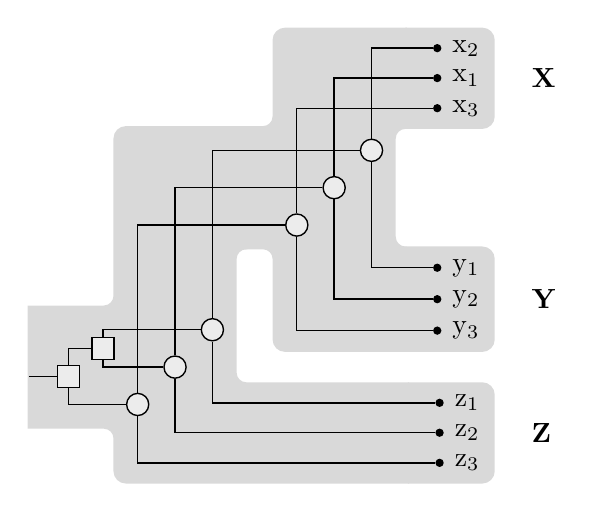
\begin{tikzpicture}
% background
\path[species background] (78.5,35.56989) [rounded corners={4pt}] -- (31.0,35.56989) -- (31.0,100.39986) [sharp corners] -- (0,100.39986) -- (0,143.89986) [rounded corners={4pt}] -- (31.0,143.89986) -- (31.0,163.71974999999998) [sharp corners] -- (136.84,163.71974999999998) -- (136.84,128.14986) [rounded corners={4pt}] -- (74.5,128.14986) -- (74.5,79.06989) [sharp corners] -- (78.5,79.06989) -- cycle;
\path[species background] (136.0,0) [rounded corners={4pt}] -- (88.5,0) -- (88.5,35.56989) [sharp corners] -- (78.5,35.56989) -- (78.5,79.06989) [rounded corners={4pt}] -- (88.5,79.06989) -- (88.5,116.14986) [sharp corners] -- (136.0,116.14986) -- (136.0,79.06989) [rounded corners={4pt}] -- (132.0,79.06989) -- (132.0,35.56989) [sharp corners] -- (136.0,35.56989) -- cycle;
\path[
                species background,
                rounded corners={4pt},
            ] (136.0,0) -- (167.763,0) -- node[species label] {X} (167.763,35.56989) -- (136.0,35.56989);
\path[
                species background,
                rounded corners={4pt},
            ] (136.0,79.06989) -- (167.763,79.06989) -- node[species label] {Y} (167.763,116.14986) -- (136.0,116.14986);
\path[
                species background,
                rounded corners={4pt},
            ] (136.84,128.14986) -- (167.763,128.14986) -- node[species label] {Z} (167.763,163.71974999999998) -- (136.84,163.71974999999998);
% species
% gene branches
\draw[branch={reccolor0}] (78.5,70.81989) -| (39.25,131.39986) (39.25,139.89986) |- (136.84,156.74477499999998);
\draw[branch={reccolor0}] (78.5,57.31989) -| (52.75,117.89985999999999) (52.75,126.39985999999999) |- (136.84,145.86481499999996);
\draw[branch={reccolor0}] (78.5,43.81989) -| (66.25,104.39985999999999) (66.25,112.89985999999999) |- (136.84,135.05484499999997);
\draw[branch={reccolor0}] (48.5,122.14985999999999) -| (26.75,111.14985999999999) (26.75,119.64985999999999) |- (62.0,108.64985999999999);
\path[branch={reccolor0}] (10.0,125.52485999999999) -- (0,125.52485999999999);
\draw[branch={reccolor0}] (35.0,135.64986) -| (14.25,121.27485999999999) (14.25,129.77486) |- (22.5,115.39985999999999);
\path[branch={reccolor0}] (92.5,70.81989) -- (78.5,70.81989);
\draw[branch={reccolor0}] (136.0,28.594915) -| (96.75,66.56989) (96.75,75.06989) |- (136.0,108.969865);
\path[branch={reccolor0}] (106.0,57.31989) -- (78.5,57.31989);
\draw[branch={reccolor0}] (136.0,17.714955) -| (110.25,53.06989) (110.25,61.56989) |- (136.0,97.609875);
\path[branch={reccolor0}] (119.5,43.81989) -- (78.5,43.81989);
\draw[branch={reccolor0}] (136.0,6.904985) -| (123.75,39.56989) (123.75,48.06989) |- (136.0,86.249885);
\path[branch={reccolor0}] (146.0,28.594915) -- (136.0,28.594915);
\path[branch={reccolor0}] (146.0,17.714955) -- (136.0,17.714955);
\path[branch={reccolor0}] (146.0,6.904985) -- (136.0,6.904985);
\path[branch={reccolor0}] (146.0,108.96986500000001) -- (136.0,108.969865);
\path[branch={reccolor0}] (146.0,97.609875) -- (136.0,97.609875);
\path[branch={reccolor0}] (146.0,86.249885) -- (136.0,86.249885);
\path[branch={reccolor0}] (146.84,156.74477499999998) -- (136.84,156.74477499999998);
\path[branch={reccolor0}] (146.84,145.864815) -- (136.84,145.86481499999996);
\path[branch={reccolor0}] (146.84,135.054845) -- (136.84,135.05484499999997);
% gene transfers
% events
\node[speciation={reccolor0}] at (39.25,135.64986) {};
\node[speciation={reccolor0}] at (52.75,122.14985999999999) {};
\node[speciation={reccolor0}] at (66.25,108.64985999999999) {};
\node[duplication={reccolor0}] at (26.75,115.39985999999999) {};
\node[duplication={reccolor0}] at (14.25,125.52485999999999) {};
\node[speciation={reccolor0}] at (96.75,70.81989) {};
\node[speciation={reccolor0}] at (110.25,57.31989) {};
\node[speciation={reccolor0}] at (123.75,43.81989) {};
\node[extant gene={reccolor0}{x\textsubscript{3}}] at (147.5,28.594915) {};
\node[extant gene={reccolor0}{x\textsubscript{1}}] at (147.5,17.714955) {};
\node[extant gene={reccolor0}{x\textsubscript{2}}] at (147.5,6.904985) {};
\node[extant gene={reccolor0}{y\textsubscript{3}}] at (147.5,108.96986500000001) {};
\node[extant gene={reccolor0}{y\textsubscript{2}}] at (147.5,97.609875) {};
\node[extant gene={reccolor0}{y\textsubscript{1}}] at (147.5,86.249885) {};
\node[extant gene={reccolor0}{z\textsubscript{3}}] at (148.34,156.74477499999998) {};
\node[extant gene={reccolor0}{z\textsubscript{2}}] at (148.34,145.864815) {};
\node[extant gene={reccolor0}{z\textsubscript{1}}] at (148.34,135.054845) {};
\end{tikzpicture}
